\documentclass[12pt]{article}
\usepackage[italian]{babel}
\usepackage{array}
\usepackage[margin=2.5cm]{geometry}
\usepackage{hyperref}
\usepackage{pdfpages}
\usepackage{xcolor}
\usepackage{subfigure}
\usepackage{amsmath}
\usepackage{relsize}
\usepackage{amsfonts}
\usepackage{subcaption}
\usepackage{graphicx}
\usepackage{listings}

\begin{document}

    \begin{titlepage}
        \centering
      
        
        {\Large Università degli Studi di Udine} \\[0.5cm]
        {\large Dipartimento di Scienze Matematiche, Informatiche e Fisiche} \\[2cm]
        
        
\includegraphics[width=0.35\textwidth]{img/uniud-logo.pdf} \\[2cm]
        
        {\Large \textbf{Progetto di Internet of Things}} \\[2cm]
        {\Large \textsc{Simulazione di un sistema per la raccolta dati e il monitoraggio operativo di macchinari industriali}} \\[3cm]

        \large 168062 - Rumiato Joshua \\
        \large rumiato.joshua@spes.uniud.it

        \vfill

        {\large Anno Accademico 2025/2026} \\[0.3cm]
        
        
    \end{titlepage}

    \newpage
    \tableofcontents
    \newpage

    \section{Introduzione}
    
    La presente relazione rielabora ed evolve parte del lavoro svolto durante il periodo di tirocinio curricolare presso una importante azienda manifatturiera del territorio.
    Il documento descrive le fasi del lavoro che vanno dalla definizione dei requisiti fino alla pianificazione della strategia di rilascio, ponendo l'accento sulla fase di configurazione e di distribuzione dei servizi necessari al funzionamento dell'architettura.
    
    \subsection{Obiettivo}
    
    L'obiettivo del progetto è la messa in opera di un'infrastruttura a basso costo, resiliente e scalabile, capace di standardizzare l'acquisizione dati in fabbrica. Nello specifico, il sistema permette di raccogliere, tramite lo standard industriale \textsc{opc ua}, i dati di operatività provenienti da macchinari produttivi eterogenei e di renderli fruibili attraverso moderni strumenti di visualizzazione e monitoraggio.
    
    \subsection{Scenario applicativo}
    
    La base del progetto, ovvero il lavoro svolto durante il tirocinio, si inserisce in un contesto industriale in cui, pur essendo stata definita un'interfaccia standard basata su \textsc{opc ua} per garantire interoperabilità tra impianti di diversi fornitori, si riscontra ancora una limitata o frammentata diffusione sul campo. Questa situazione rende il progetto strategico per due motivazioni principali:
    \begin{itemize}
        \item promuove e accelera il processo di adozione dello standard di interoperabilità;
        \item definisce un flusso che trasforma dati grezzi in informazioni facilmente fruibili.
    \end{itemize}
    
    \subsection{Requisiti e funzionalità}
    
    La realizzazione del sistema in oggetto parte da un ristretto insieme di requisiti generici emersi nelle fasi iniziali delle attività:
    \begin{itemize}
        \item il sistema deve monitorare le variazioni degli stati operativi dei macchinari tramite una sottoscrizione \textsc{opc ua}, così da alleggerire il carico sulla rete aziendale;
        \item i dati letti vanno salvati su un supporto centralizzato che supporti le \textit{time-series};
        \item lo storico delle variazioni va utilizzato per la costruzione di una \textit{dashboard} che riporti sintesi di interesse sugli intervalli temporali scelti dagli utenti;
        \item la perdita di informazioni dovuta a disservizi di rete non è considerata critica. 
    \end{itemize}
    
    In fase di sviluppo, al fine di rispondere a necessità emergenti e per garantire la massima estensibilità del sistema, sono state aggiunte ulteriori funzionalità:
    \begin{itemize}
        \item pubblicazione dei dati in tempo reale via protocollo \textsc{mqtt};
        \item \textit{logging} e tracciamento su piattaforma centralizzata per l'osservabilità;
        \item integrazione e comunicazione con il sistema gestionale/\textsc{mes} aziendale per la correlazione dei dati di produzione con la telemetria di campo.
    \end{itemize}
    
    \subsection{Struttura del documento}
    Il resto della relazione illustrerà dapprima un quadro di nozioni e tecnologie abilitanti, per poi descrivere le scelte progettuali compiute e i dettagli implementativi all'interno delle sezioni dedicate. La trattazione si conclude analizzando la strategia di rilascio del software sviluppato, discutendo in ultimo luogo le conclusioni su quanto realizzato al fine di evidenziare possibili sviluppi futuri per il progetto.

    \section{Quadro teorico}

    \subsection{OPC UA}
    
    Acronimo di \textit{Open Platform Communications Unified Architecture}, è uno standard \textit{platform-independent} e \textit{open-source} progettato per la comunicazione e l'interoperabilità industriale in ottica IoT e Industria 4.0. 
    Esso organizza le informazioni in uno spazio di indirizzi strutturato ad albero (\textit{Address Space}) in cui ogni elemento (nodo) include non solo il dato grezzo, ma anche metadati, proprietà e relazioni semantiche. 
    Lo standard supporta sia paradigmi di comunicazione tradizionali di tipo \textit{client-server} sia modelli orientati agli eventi di tipo \textit{publish-subscribe}, implementando nativamente meccanismi di sicurezza quali la crittografia dei canali e l'autenticazione dei dispositivi.
    
    \subsection{MQTT}
    
    Protocollo di messaggistica leggero di tipo \textit{publish-subscribe} basato su architettura \textsc{tcp/ip}, ottimizzato per contesti con risorse hardware limitate o reti instabili (scenari IoT ed \textit{edge}). 
    L'architettura prevede al centro della comunicazione un'entità denominata \textit{broker}, incaricata di gestire lo scambio dei messaggi tra i \textit{publisher} (client che generano e inviano i dati su specifici \textit{topic} gerarchici) e i \textit{subscriber} (client che ricevono i dati registrandosi a tali canali). 
    La robustezza e l'affidabilità della consegna sono regolate dalla \textit{Quality of Service} (QoS), definita su tre livelli crescenti: QoS 0 (consegna \textit{at most once}), QoS 1 (consegna \textit{at least once}) e QoS 2 (consegna \textit{exactly once}).
    
    \subsection{Database time-series}
    
    Si tratta di sistemi di gestione di basi di dati ottimizzati per serie temporali, specializzati quindi nell'archiviazione e nell'elaborazione di sequenze di dati campionati nel tempo. 
    A differenza delle basi di dati relazionali tradizionali, garantiscono elevate prestazioni di ingestione dati in presenza di flussi continui e risposte rapide a \textit{query} analitiche complesse. Questo è reso possibile da ottimizzazioni specifiche a livello di \textsc{i/o}, dall'indicizzazione cronologica, dal \textit{chunking} (partizionamento) dei dati e dalla definizione automatizzata di \textit{policy} di compressione e ritenzione dei dati.
    
    \subsection{Osservabilità}
    
    Nel contesto dei sistemi distribuiti, l'osservabilità definisce la capacità di comprendere e inferire lo stato interno di un'infrastruttura analizzando esclusivamente i dati prodotti in output da essa. 
    Un approccio orientato all'osservabilità semplifica le attività di manutenzione software, riducendo drasticamente il tempo medio di risoluzione dei disservizi. Tale paradigma si fonda su tre pilastri fondamentali:
    \begin{itemize}
        \item \textbf{metriche}: dati numerici aggregati e campionati nel tempo utili per valutare lo stato di salute generale del sistema;
        \item \textbf{\textit{log}}: registri testuali emessi per descrivere eventi specifici, avvisi o anomalie;
        \item \textbf{tracce}: ricostruzioni dettagliate del percorso e delle dipendenze causali di una richiesta attraverso i microservizi dell'architettura.
    \end{itemize}

    \subsection{Portabilità e Containerizzazione}
    
    La portabilità rappresenta la capacità di un'applicazione software di essere eseguita su infrastrutture hardware e sistemi operativi differenti senza richiedere modifiche al codice sorgente. Nelle moderne architetture software, questo requisito viene soddisfatto principalmente tramite le tecnologie di containerizzazione, che permettono di racchiudere codice, librerie, e \textit{runtime} delle applicazioni in un ambiente isolato e standardizzato.
    
    A differenza delle tradizionali macchine virtuali, i \textit{container} condividono il kernel del sistema operativo ospitante, risultando più leggeri e veloci nell'avvio. 
    Questo consente una maggiore efficienza nell'utilizzo delle risorse e facilita operazioni di distribuzione, aggiornamento e scalabilità dei servizi.
    
    La containerizzazione viene inoltre ampiamente utilizzata nei processi di \textit{Continuous Integration} e \textit{Continuous Deployment} (CI/CD).
    Attraverso i \textit{container}, infatti, è possibile eseguire automaticamente compilazione, test e distribuzione delle applicazioni riutilizzando le configurazioni e aumentando l'affidabilità delle procedure di rilascio.

    \section{Progettazione}
    \subsection{Architettura}

    \begin{center}
        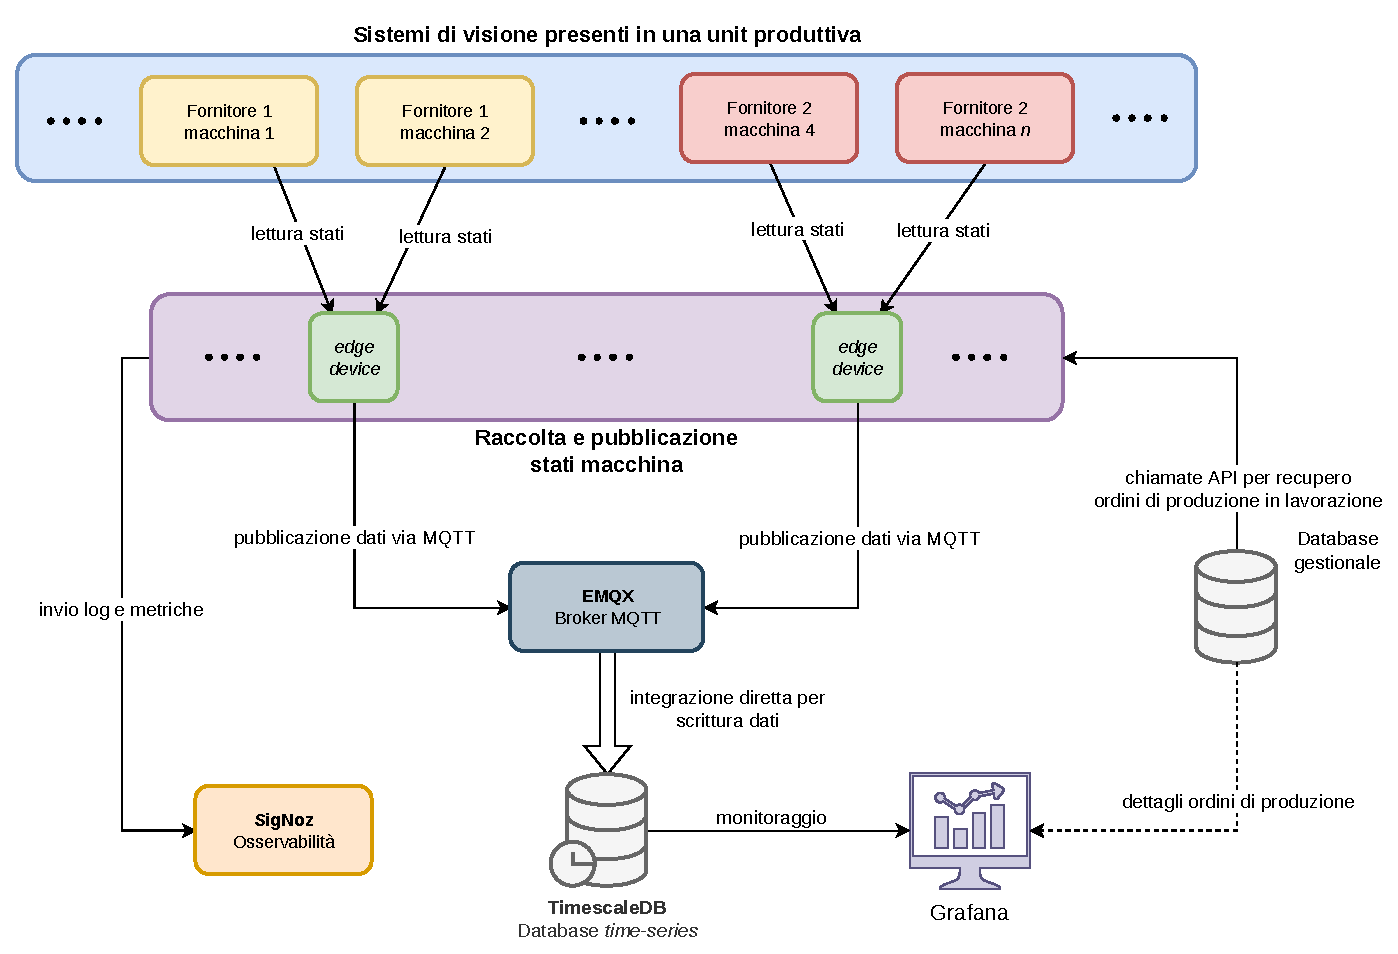
\includegraphics[
            angle=90,
            width=\textheight,
            height=\dimexpr\textheight-2cm\relax,
            keepaspectratio
        ]{img/architecture.pdf}
    \end{center}
    
    \paragraph{Dispositivi \textit{edge}} Il cuore dell'architettura proposta consiste in una flotta di dispositivi con la funzione di \textit{gateway} tra il dominio \textit{Operational Technology} (\textsc{ot}), ossia il parco macchinari, e l'infrastruttura \textsc{it}.
    
    I dispositivi, configurati per l'installazione in prossimità delle macchine (da cui la dicitura \textit{edge}), assolvono tre funzioni principali, gestite interamente in modo asincrono per ottimizzare l'uso delle risorse hardware ed evitare colli di bottiglia nell'elaborazione dei flussi di \textsc{i/o}:
    \begin{itemize}
        \item \textbf{acquisizione}: sottoscrizione alle variazioni dei nodi relativi agli stati macchina esposti dai server \textsc{opc ua} integrati a bordo dei macchinari (in conformità con lo standard descritto nell'introduzione);
        \item \textbf{integrazione}: arricchimento dei dati di campo con richieste \textsc{http} mirate alle \textsc{api} che si interfacciano con il sistema gestionale/\textsc{mes}, consentendo di correlare telemetria dei macchinari e contesto operativo;
        \item \textbf{pubblicazione}: le informazioni ottenute dalle fasi precedenti vengono serializzate in formato \textsc{json} e pubblicate via \textsc{mqtt}, utilizzando \textit{topic} gerarchici specifici per ogni macchinario di campo.
    \end{itemize}

    Per garantire l'affidabilità su hardware e risorse limitate, l'implementazione segue criteri di tolleranza ai guasti di rete e di ottimizzazione degli accessi alle memorie di massa. In particolare, per preservare l'integrità delle schede \textsc{sd} utilizzate su eventuali nodi Raspberry Pi, sono state adottate le seguenti misure:
    \begin{itemize}
        \item disabilitazione della partizione \textit{swap} del sistema operativo (non attuata nella simulazione);
        \item predisposizione del codice per l'esecuzione in \textit{container} configurati in sola lettura;
        \item inoltro dei \textit{log} verso una piattaforma di osservabilità remota.
    \end{itemize}

    La containerizzazione consente inoltre di ospitare più \textit{gateway} a bordo di un singolo dispositivo fisico, assicurando flessibilità nella gestione dei carichi di lavoro.

    \paragraph{Broker MQTT e persistenza}

    La gestione della messaggistica è affidata al broker \textsc{emqx}, scelto per l'elevata scalabilità, le prestazioni e la capacità di gestire nativamente l'inoltro dei dati ricevuti verso sistemi di \textit{storage} attraverso un motore di regole integrato.
    
    Inoltre, grazie alla predisposizione per l'utilizzo di connessioni crittografate tramite \textsc{tls}, \textsc{emqx} può garantire un ottimo livello di sicurezza nella trasmissione dei dati.
    
    Una volta ricevuti dal \textit{broker} e inoltrati, i dati vengono memorizzati in un'istanza TimescaleDB, estensione di PostgreSQL ottimizzata per serie temporali tramite l'uso di tabelle partizionate temporalmente chiamate \textit{hypertables}. Questa scelta garantisce una copertura ottimale dei requisiti del progetto e piena interoperabilità con il linguaggio \textsc{sql} standard e gli strumenti già a disposizione nella realtà di riferimento. 

    \paragraph{Monitoraggio e osservabilità}
    Monitoraggio e visualizzazione sono affidati a Grafana, scelto per l'efficienza nella gestione di serie temporali e per l'integrazione nativa con PostgreSQL/TimescaleDB.

    L'ecosistema di osservabilità è gestito mediante SigNoz, strumento \textit{open-source} completo per l'osservabilità, utilizzato per il \textit{logging} dei server \textsc{opc ua} a bordo dei macchinari, dei \textit{gateway} e del server \textsc{http} che risponde alle chiamate \textsc{api} verso il gestionale/\textsc{mes}. La centralizzazione dei \textit{log} è stata voluta non solo per ridurre l'usura dei supporti di memoria dei dispositivi, ma anche per facilitare la diagnosi remota e la risoluzione di disservizi.
    
    \subsection{Modello dei dati}

    \subsubsection{Formato messaggi}

    Mentre la lettura degli stati macchina tramite \textsc{opc ua} è regolata dalle specifiche dello standard in questione, il \textit{payload} generato dai dispositivi \textit{edge} e pubblicato sul \textit{broker} viene strutturato in formato \textsc{json}. Tale scelta trova motivazione nella flessibilità offerta dal formato, oltre che nella facilità di \textit{parsing} automatico da parte di \textsc{emqx}.

    Ogni messaggio, che notifica la variazione di uno stato macchina, include i seguenti campi:
    \begin{itemize}
        \item \verb|timestamp|: marcatura temporale in formato \textit{Unix epoch} generata al momento della ricezione della variazione;
        \item \verb|machine_id|: identificativo univoco del macchinario che ha generato l'evento;
        \item \verb|variable|: nome del nodo \textsc{opc ua} di cui si è registrata la variazione;
        \item \verb|type|: tipo del nodo \textsc{opc ua} di cui si è registrata la variazione;
        \item \verb|value|: valore del nodo \textsc{opc ua} di cui si è registrata la variazione;
        \item \verb|order_id|: identificativo dell'ordine di produzione prelevato dal sistema gestionale/\textsc{mes}.
    \end{itemize}

    \subsubsection{Pubblicazione}

    L’organizzazione dei topic \textsc{mqtt} segue un formato che assicura uniformità e facilità nella gestione. La struttura adottata è la seguente: \verb|ambiente/servizio/id_macchinario|.
    
    Questa convenzione minimizza il numero di livelli necessari all'interno del topic, pur consentendo di distinguere i flussi di messaggi in transito sul \textit{broker} in funzione dell'ambiente di esecuzione (\textit{test}, \textit{staging}, \textit{produzione}, \dots) e del servizio associato. In questo modo viene minimizzato il rischio di conflitti con altre applicazioni che utilizzano il medesimo \textit{broker}.

    \subsubsection{Persistenza}
    
    Per agevolare le operazioni di \textit{storage}, si mantiene lo schema della tabella in cui verrà salvato lo storico delle variazioni analogo a quello del \textsc{json} inviato tramite \textsc{mqtt}.

    Come già anticipato, l'adozione delle \textit{hypertable} TimescaleDB semplifica le operazioni sulla base di dati e le successive analisi.
    
    
    \section{Sviluppo e implementazione}
    \subsection{Gateway OPCUA-MQTT}
    Il codice dei dispositivi \textit{edge} è stato sviluppato in Python e pensato per essere eseguito all'interno di un \textit{container} Docker, leggendo i parametri di configurazione da appositi file \verb|.env|. La flessibilità operativa viene quindi implementata ricorrendo al dispiegamento di tante istanze indipendenti dell'applicazione quante sono le attrezzature da monitorare.

    Il sorgente del \textit{gateway} è stato organizzato in cinque file, seguendo principi di modularità e separazione delle responsabilità.

    \paragraph{\texttt{async\_mesapi\_client.py}} Implementa un \textit{client} asincrono basato sulla libreria \verb|aiohttp| per l'interazione con l'\textsc{api} del \textsc{mes}/gestionale per il recupero dell'ordine attivo su un macchinario. Il modulo assicura inoltre una corretta gestione del ciclo di vita della sessione \textsc{http}.

    \paragraph{\texttt{async\_mqtt\_publisher.py}} Funge da \textit{wrapper} per la libreria \verb|aiomqtt|, semplificando l'interazione con il broker \textsc{mqtt}. Il modulo automatizza la serializzazione dei \textit{payload} in formato \textsc{json} e integra il supporto nativo per la sicurezza del canale.

    \paragraph{\texttt{async\_opc\_client.py}} Implementa l'interfaccia di comunicazione con il server \textsc{opc ua} tramite la libreria \verb|asyncua|. Il modulo mantiene la connessione con il server e sottoscrive i nodi configurati, intercettando in tempo reale le loro variazioni di valore. I dati acquisiti vengono arricchiti con metadati e \textit{timestamp} prima di essere inseriti in una coda asincrona condivisa, garantendo il disaccoppiamento tra acquisizione e trasmissione

    \paragraph{\texttt{gateway\_telemetry.py}} Configura un client \textit{OpenTelemetry} per l'esportazione dei \textit{log} dell'applicazione verso un collettore remoto (SigNoz).

    \paragraph{\texttt{main.py}} Inizializza le componenti del \textit{gateway}, caricando le configurazioni dalle variabili d'ambiente, e ne gestisce il coordinamento. Il cuore del modulo è strutturato su un paradigma a produttore-consumatore basato sulla libreria \verb|asyncio|:
        \begin{itemize}
            \item \textbf{produttore} (\textsc{opc ua}): stabilisce e mantiene la connessione con il server \textsc{opc ua}. Una volta attivata la sottoscrizione ai nodi configurati, i dati variati vengono inviati a una coda asincrona condivisa di dimensione fissa, configurata per scartare i messaggi in caso di saturazione.
            \item \textbf{consumatore}: preleva i dati dalla coda condivisa, li arricchisce in tempo reale con l'ordine di produzione corrente e li trasmette al broker \textsc{mqtt} (ai fini della trattazione, la comunicazione avviene in chiaro per evitare di gestire la complessità introdotta dai certificati).
        \end{itemize}
    Il modulo implementa una gestione avanzata degli errori di rete, delle eccezioni e dei segnali di sistema (\textsc{sigint}, \textsc{sigterm}) per garantire uno \textit{shutdown} controllato delle risorse. La concorrenza è limitata da un semaforo per limitare il numero di pubblicazioni simultanee, evitando il sovraccarico delle risorse del dispositivo \textit{edge} in presenza di picchi di traffico dati.
    
    \subsection{Setup ambiente di simulazione}
    
    Mentre in ambito aziendale il \textit{gateway} si inseriva in un ecosistema di servizi già configurati, ai fini della presente trattazione è stato realizzato un ambiente di simulazione completo e integrato tramite Docker, ospitato all'interno di un sistema operativo Debian su \textsc{wsl2} (\textit{Windows Subsystem for Linux}).

    Per meglio separare le responsabilità e fronteggiare la complessità dei servizi, l'organizzazione dell'ambiente è stata suddivisa in tre macro-componenti indipendenti.
    \begin{itemize}
        \item \textbf{\textit{stack} di osservabilità}: orchestrato tramite un file \texttt{docker-compose} reperito dal \textit{repository} ufficiale GitHub, configura dei servizi necessari al funzionamento di SigNoz (come il collettore \textit{OpenTelemetry} e il database ClickHouse);
        \item \textbf{nodi di campo} (server \textsc{opc ua}): gestiti in modo granulare e indipendente per emulare in modo realistico il comportamento dinamico di un parco macchine industriale;
        \item \textbf{\textit{stack} dei servizi applicativi}: gestito mediante un secondo file \texttt{docker-compose} contenente le configurazioni di \textsc{emqx}, TimescaleDB, il servizio di generazione di dati fittizi per la base di dati, Grafana e il server \textsc{api} per \textsc{mes}/gestionale.
    \end{itemize}

    \begin{figure}[htbp]
        \centering
        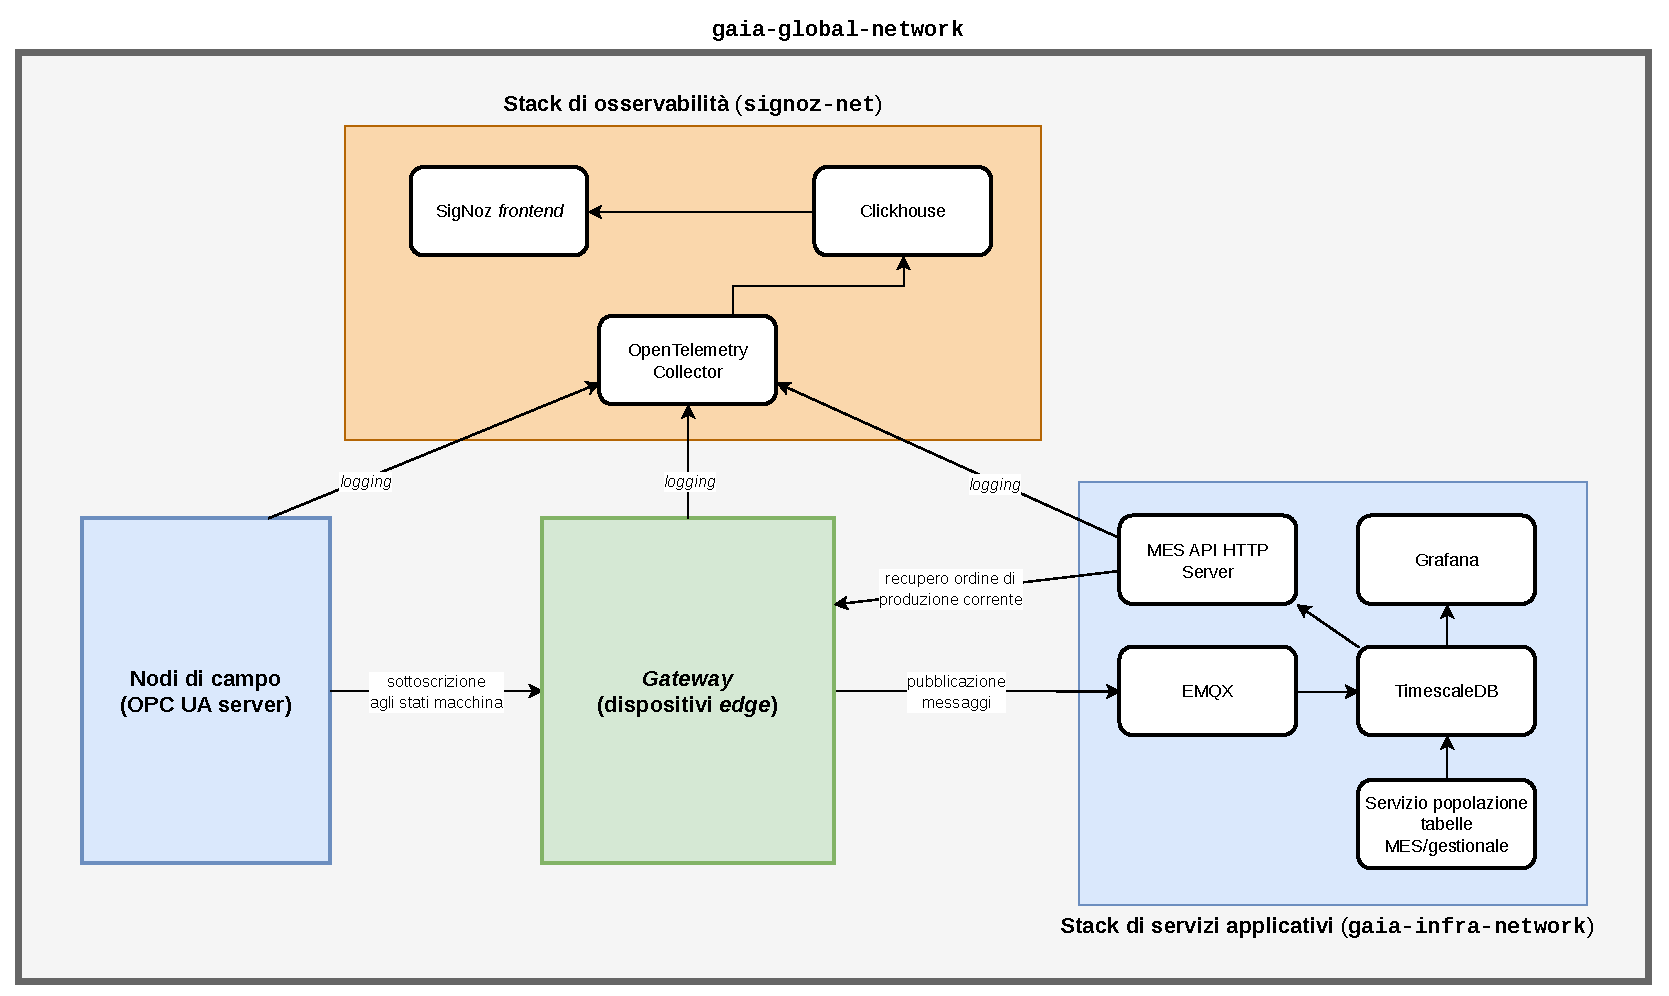
\includegraphics[width=0.9\linewidth]{img/containers.pdf}
        \caption{Architettura dell'ambiente simulato}
        \label{fig:placeholder}
    \end{figure}

    La comunicazione tra le componenti è garantita dalla previa creazione di una rete Docker chiamata \verb|gaia-global-network| con \textit{driver} \verb|bridge| isolato. Questa scelta separa il traffico della simulazione da quello della rete ospite e abilita il \textsc{dns} interno di Docker, permettendo ai \textit{container} di comunicare utilizzando stringhe logiche (i nomi dei \textit{container}) come \textit{hostname}.\newline

    Sulla scia di quanto osservato nel \verb|docker-compose| per l'osservabilità, anche l'orchestrazione dei servizi applicativi è stata integrata con meccanismi di \textit{healthcheck}. Attraverso l'uso di clausole \verb|depends_on| condizionate allo stato di salute del database, moduli come il generatore di popolazione iniziale, il server \textsc{http} e la dashboard Grafana rimangono in attesa dell'effettiva prontezza operativa di TimescaleDB prima di allocare le proprie risorse e avviare i rispettivi processi. La definizione di questi vincoli strutturali garantisce una corretta sequenza d'avvio, massimizza l'affidabilità e la resilienza dell'intero \textit{deployment}.

    \subsubsection{Stack di osservabilità}
    Attraverso poche mirate modifiche al file di configurazione standard di SigNoz, il collettore \textit{OpenTelemetry} deputato alla raccolta della telemetria viene esposto verso tutti i \textit{container} dell'infrastruttura predisposti per l'osservabilità:
    \begin{itemize}
        \item \textbf{dichiarazione delle rete globale esterna}: nella sezione radice \textit{networks} è stata inserita la rete globale, contrassegnata come \verb|external: true| per indicare l'utilizzo di una rete preesistente, non legata ai servizi definiti nel \verb|docker-compose|;
        \begin{verbatim}
        networks:
          signoz-net:
            name: signoz-net
          gaia-global-network:
            name: gaia-global-network
            external: true
        \end{verbatim}
        \item \textbf{collegamento al modulo di ricezione}: il servizio \verb|otel-collector| viene configurato come ponte tra la rete interna di SigNoz (\verb|signoz-net|) e quella adottata per l'ascolto dei messaggi provenienti dal resto dell'ambiente.
        \begin{verbatim}
          otel-collector:
            # ... various configurations ...
            networks:
              - gaia-global-network
              - signoz-net
        \end{verbatim}
    \end{itemize}
    
    \subsubsection{Server OPC UA}
    Prevedendo la configurazione di un server a bordo di ogni macchinario da monitorare, l'implementazione del codice viene strutturata in continuità con quanto fatto con i dispositivi \textit{edge}: una \textit{codebase} unica, agnostica, da poter lanciare in un numero di istanze arbitrarie.
    Il sorgente è stato organizzato in tre file.

    \paragraph{\texttt{opcua\_server.py}} Gestisce il ciclo di vita di un server \textsc{opc ua} asincrono. Espone dei dati simulando la struttura gerarchica di un \textit{namespace} con all'interno quattro tag booleani rappresentanti possibili stati macchina:
    \begin{itemize}
        \item \textbf{\textit{InAlarm}}: segnala la presenza di una condizione di lavoro bloccante (anomalia o errore) che richiede intervento immediato;
        \item \textbf{\textit{InBypass}}: denota l'operatività del macchinario, ma con alcune funzionalità di controllo o sicurezza disabilitate;
        \item \textbf{\textit{InCycle}}: indica la piena operatività del macchinario;
        \item \textbf{\textit{InWarning}}: segnala la presenza di una condizione di lavoro non bloccante, ma che richiede monitoraggio.
    \end{itemize}
    
    \paragraph{\texttt{opcua\_server\_telemetry.py}} Similmente a \texttt{gateway\_telemetry.py}, implementa le funzionalità di osservabilità, la configurazione di un client \textit{OpenTelemetry} e l'integrazione con il modulo \verb|logging| di Python per l'invio di \textit{log} ad un collettore remoto.
 
    \paragraph{\texttt{main.py}} Costituisce l'\textit{entry point} dell'applicazione, orchestrando l'inizializzazione della telemetria, del server e la simulazione del comportamento dinamico di un macchinario industriale. Quest'ultima funzionalità viene eseguita in \textit{background} tramite la libreria \verb|asyncio|.

    \subsubsection{Popolazione database gestionale/MES}

    Per garantire il corretto funzionamento delle \textsc{api} utilizzate dai \textit{gateway} è stato realizzato un modulo in grado di popolare il database con dati deterministici, riproducibili e realistici, simulando un ambiente produttivo che traccia ordini, articoli e dichiarazioni di avanzamento.

    Nel contesto dell'ambiente simulato, il modulo è stato progettato come un servizio temporaneo denominato \verb|fill-db-service|, associato al profilo Docker \verb|init| e configurato con la direttiva \verb|restart: "no"|. Questo garantisce che il servizio venga avviato solo quando esplicitamente dichiarato e si arresti definitivamente una volta completata la scrittura nelle tabelle.
    
    La struttura logica della base di dati simulata segue quanto illustrato di seguito:
    \begin{lstlisting}[breaklines=true, basicstyle=\ttfamily\small, columns=fullflexible]
        articles [ id (PK), description ]
        orders   [ id (PK), article_id (FK), machine_id, target_qty, start_date, end_date ]
        order_progress_statements [order_id (PK, FK), timestamp (PK), produced_qty, discarded_qty ]
    \end{lstlisting}

    \begin{figure}[htbp]
        \centering
        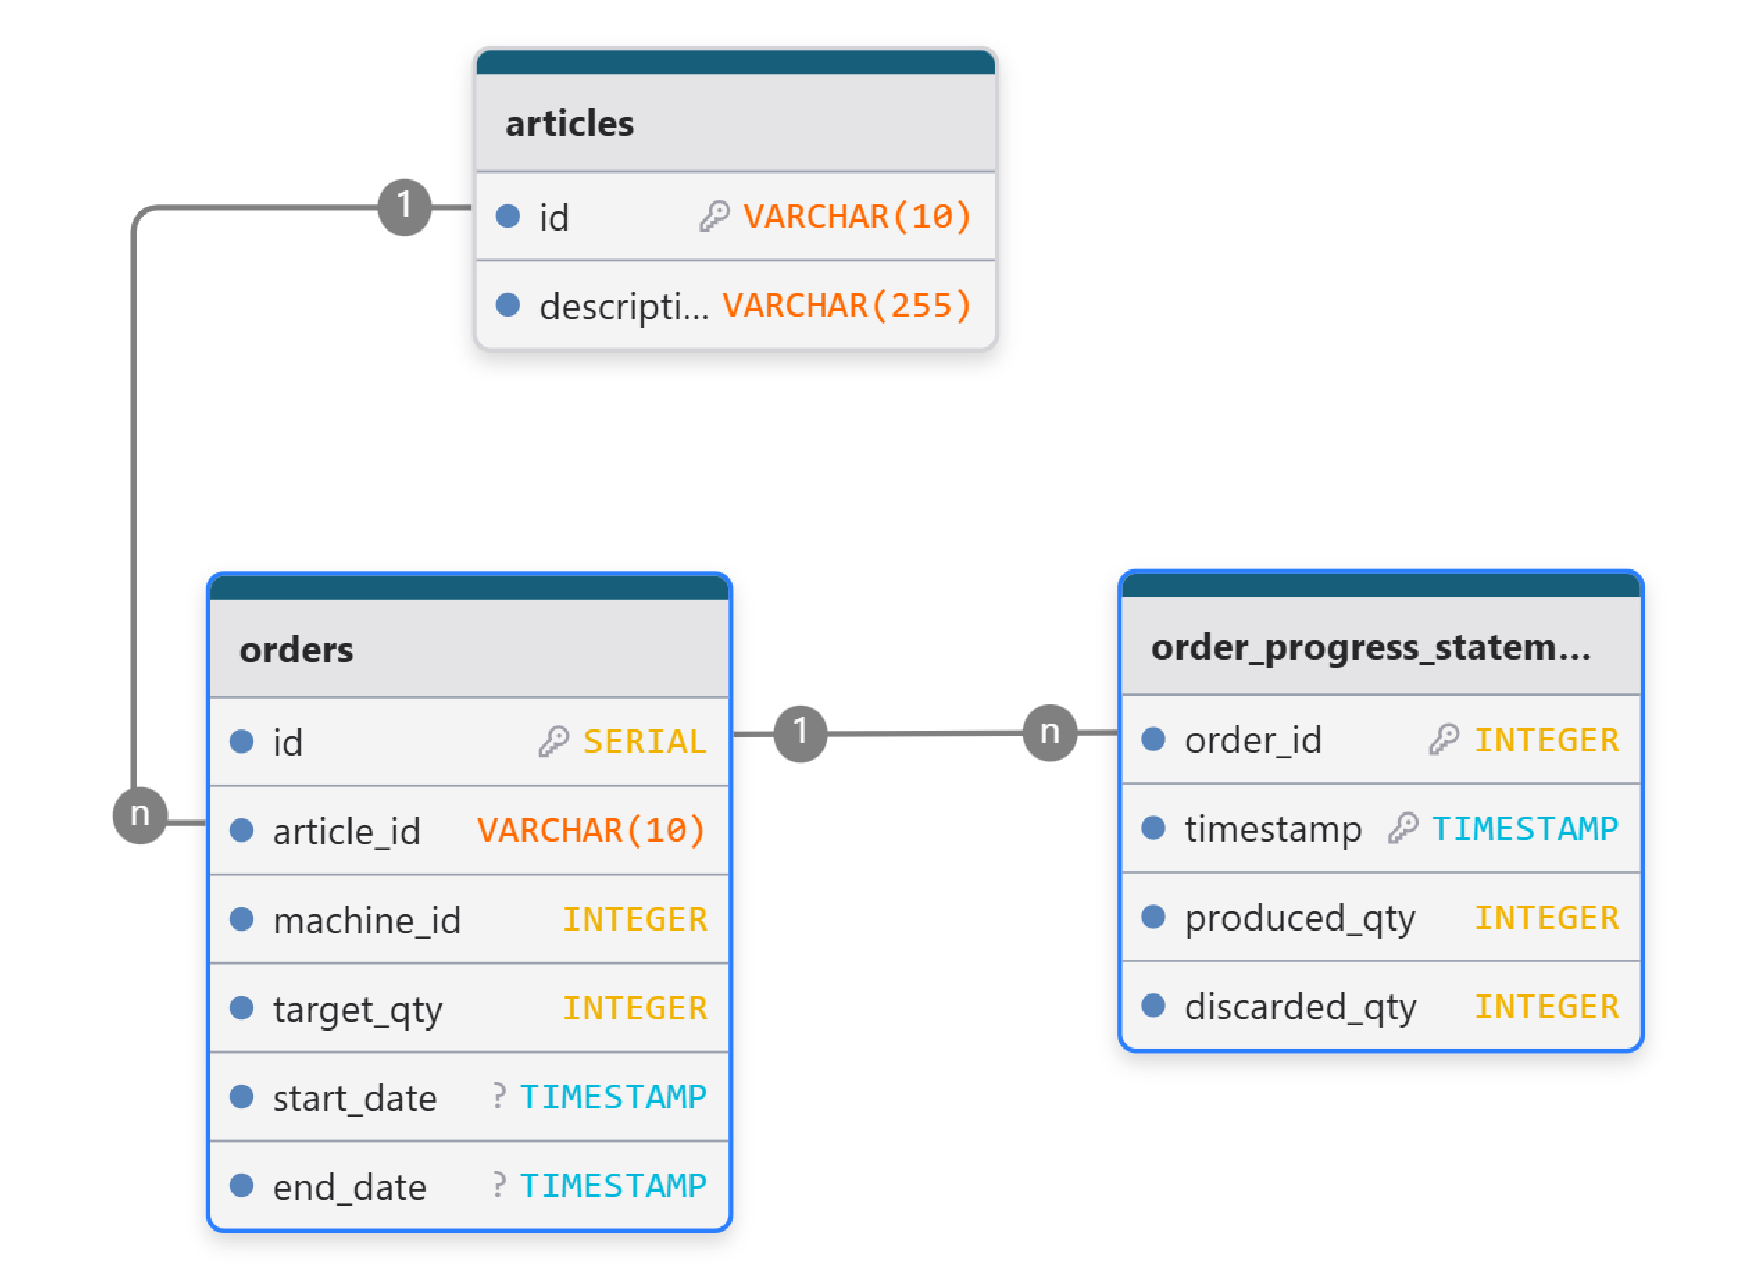
\includegraphics[width=0.7\linewidth]{img/dbschema.pdf}
        \caption{Schema delle tabelle del \textsc{mes}/gestionale}
    \end{figure}
    
    Non potendo riprodurre fedelmente il funzionamento di un ambiente produttivo reale in tutta la sua complessità, l'algoritmo di popolazione si basa sui seguenti vincoli operativi e semplificazioni di modello:
    \begin{itemize}
        \item ogni ordine di produzione viene allocato a una singola macchina per l’intera durata della sua esecuzione;
        \item ogni macchinario elabora un singolo ordine alla volta, escludendo elaborazioni parallele;
        \item i macchinari sono modellati per essere costantemente occupati nella produzione, eventuali tempi morti non sono tracciati;
        \item le quantità prodotte e scartate ad ogni dichiarazione di avanzamento sono incrementali rispetto alla precedente rilevazione;
        \item un ordine di produzione è considerato concluso non appena la differenza tra la somma delle quantità prodotte e quella delle quantità scartate è maggiore o uguale alla quantità \textit{target} pianificata
    \end{itemize}
     L'intero codice del servizio è stato strutturato nei file descritti.
    
    \paragraph{\texttt{config.py}} Definisce i parametri operativi, i \textit{seed} per la riproducibilità e le specifiche di prodotti e macchine. Sono stati configurati 5 macchinari, aventi i seguenti \textsc{id}: 1123, 3311, 5563, 7742, 9987.

    \paragraph{\texttt{database\_connection.py}} Gestisce il ciclo di vita della connessione al database PostgreSQL e l'esecuzione di query singole o in \textit{batch}.

    \paragraph{\texttt{main.py}} Coordina l'intera logica di popolamento attraverso un algoritmo strutturato in cinque fasi:
    \begin{itemize}
        \item \textbf{creazione schema}: inizializza la base di dati creando le tabelle (con relativi attributi e vincoli di integrità) e gli indici;
        \item \textbf{generazione articoli}: inserisce nell'anagrafica dei prodotti gli identificativi e le descrizioni di 20 prodotti, come definiti nel file di configurazione;
        \item \textbf{generazione ordini}: crea 100 ordini per ogni articolo, distribuiti tra 5 macchinari, con logica \textit{round-robin} e quantità variabile di multipli di 500 nell'intervallo $[9000;15000]$;
        \item \textbf{simulazione avanzamenti}: per ogni ordine, genera una cronologia di avanzamenti di produzione, simulando intervalli tra le dichiarazioni di 10-20 minuti e quantità variabili uniformemente nell'intervallo $[90;150]$, applicando al contempo una percentuale di scarto casuale nel \textit{range} $[0;1.5]$;
        \item \textbf{calcolo date}: per ogni ordine, osserva i \textit{timestamp} della prima e dell'ultima dichiarazione per determinare retroattivamente i campi \verb|start_date| e \verb|end_date| della tabella \verb|orders|.
    \end{itemize}
    
    \subsubsection{Interazione con la base di dati}

    Il servizio di \textit{backend}  per le chiamate \textsc{http} è stato realizzato in Python  (in continuità tecnologica con il resto del progetto) attraverso il \textit{framework} \verb|fastapi|, predisposto per l'invio di telemetria remota e configurato per per offrire due \textit{endpoint}:
    \begin{itemize}
         \item \verb|/health|: \textit{endpoint} operativo utilizzato per verificare lo stato di attività del servizio;
         \item \verb|/active-order-id|: richiede il parametro \verb|machine| (\textsc{id} macchinario) e restituisce il numero d'ordine di produzione attivo all'istante della chiamata sul macchinario indicato.
    \end{itemize}

    Il codice risulta strutturato nei file che seguono.
    
    \paragraph{\texttt{main.py}} Espone gli \textit{endpoint}, implementa la gestione del sistema di telemetria e la logica dell'applicativo (integrazione con la base di dati tramite \verb|sqlalchemy| con relativa elaborazione dei risultati)

    \paragraph{\texttt{mesapi\_server\_telemetry.py}} Invia i \textit{log} sullo stato del server e delle chiamate (ed i risultati) ad un collettore remoto basato su \textit{OpenTelemtry} (\textsc{otel}).

    \subsection{Persistenza dei dati}
    
    Il tracciamento dell'evoluzione degli stati macchina nel tempo avviene mediante l'integrazione nativa tra il broker e una \textit{hypertable} TimescaleDB, creando un regola di \textit{data bridge} che mappa i campi del payload \textsc{json} dei messaggi \textsc{mqtt} allo schema della tabella di destinazione.

    La definizione di questa regola richiede la previa configurazione del supporto persistente. Viene quindi creata una tabella \verb|machine_status_changes|, progettata secondo le specifiche precedentemente definite per accogliere i dati operativi necessari al monitoraggio simultaneo di molteplici nodi e macchinari.
    
    \begin{table}[htbp]
        \centering
        \caption{Schema della tabella \texttt{machine\_status\_changes}}
        \label{tab:schema_database}
        \begin{tabular}{lll}
            \hline
            \textbf{Attributo} & \textbf{Tipo di dato} & \textbf{Vincoli} \\ \hline
            \verb|timestamp|   & \verb|TIMESTAMP|   & \verb|NOT NULL| \\
            \verb|machine_id|  & \verb|INTEGER|       & \verb|NOT NULL| \\
            \verb|variable|    & \verb|VARCHAR(20)|   & \verb|NOT NULL| \\
            \verb|type|        & \verb|VARCHAR(20)|   & \verb|NOT NULL| \\
            \verb|value|       & \verb|INTEGER|       & \verb|NOT NULL| \\
            \verb|order_id|    & \verb|INTEGER|       & \verb|-| \\ \hline
        \end{tabular}
    \end{table}
    
    
    In riferimento alla tabella \ref{tab:schema_database} si noti che:
    \begin{itemize}
        \item nonostante gli stati macchina vengano modellati con valori booleani, si è deciso di assegnare a \verb|value| tipo intero per predisporre il sistema ad evoluzioni future (come le letture di contapezzi).
        \item il campo \verb|order_id| è l'unico a permettere valori nulli. Ciò garantisce che ogni messaggio venga salvato anche in caso di indisponibilità momentanea del servizio \textsc{api} durante la fase di arricchimento del dato.
    \end{itemize}

    In TimescaleDB, l'ottimizzazione per i carichi di lavoro \textit{time-series} avviene tramite la conversione della tabella appena creata in una \textit{hypertable}. Questa astrazione permette di suddividere automaticamente i dati in \textit{chunk} (partizioni fisiche) basati sul tempo, migliorando l'efficienza degli indici e la velocità di inserimento. La trasformazione viene eseguita invocando la funzione \verb|create_hypertable()|, specificando la tabella \textit{target} e la colonna temporale da utilizzare come chiave di partizionamento:
    
    \begin{verbatim}
        SELECT create_hypertable('machine_status_changes', 'timestamp');
    \end{verbatim}
    
    L'effettiva creazione e lo stato della \textit{hypertable} possono essere verificati tramite interrogazione alla vista di sistema \verb|timescaledb_information.hypertables|. Sebbene la dimensione di ogni \textit{chunk} sia stata mantenuta sul valore predefinito di 7 giorni, è stata impostata una \textit{retention policy} di 13 mesi per consentire futuri confronti analitici tra periodi omologhi su base annuale. \newline

    \begin{verbatim}
        SELECT add_retention_policy(
            'machine_status_changes',
            drop_after => INTERVAL '13 months'
        );
    \end{verbatim}

    A questo punto, per finalizzare le procedure di persistenza dei dati, sono state compiute due operazioni di configurazione su \textsc{emqx}.

    La prima, più immediata ma non meno importante, è stata la definizione di un meccanismo di autenticazione basato su \textit{username} e \textit{password} per autenticare i \textit{publisher} e fornire un maggior livello di protezione.
    Pur esistendo altri metodi di autenticazione, si è scelto questo per il compromesso offerto tra semplicità e sicurezza nell'ambiente di riferimento.
    
    A seguire, sono state configurate l'intercettazione dei messaggi pubblicati sui \textit{topic} relativi al monitoraggio e la conseguente operazione di scrittura su \verb|machine_status_changes|.
    La prima avviene attraverso un'interrogazione in linguaggio \textit{\textsc{sql}-like}, che preleva le informazioni di interesse dai messaggi ricevuti sotto i \textit{topic} che presentano il prefisso specificato. L'utilizzo del carattere \textit{jolly} \verb|#| consente di effettuare una sottoscrizione multi-livello, che raccoglie indistintamente i messaggi provenienti da qualsiasi macchinario eliminando la necessità di definire una \textit{query} specifica per ognuno di questi.
    
    \begin{verbatim}
    SELECT 
      payload.timestamp as timestamp,
      payload.machine_id as machine_id,
      payload.variable as variable, 
      payload.type as type,
      payload.value as value, 
      payload.order_id as order_id
    FROM "prod/gaia/#"
    \end{verbatim}
    
    L'output della regola di intercettazione è collegato a un \textit{Sink} configurato per interagire con l'istanza PostgreSQL/TimescaleDB.  In questa fase, oltre alla connessione verso il database (\textit{host}, porta, nome della base di dati e credenziali di accesso), viene utilizzata una \textit{prepared statement} parametrizzata per l'inserimento dei dati. Sempre in questa fase avviene la conversione del \textit{timestamp} dal formato \textit{Unix epoch} a quello compatibile con il tipo \verb|TIMESTAMP| di PostgreSQL.
    
    \begin{verbatim}
        INSERT INTO machine_status_changes (
          timestamp, machine_id, variable, type, value, order_id
        ) 
        VALUES (
          (CASE 
            WHEN ${variable} = 'DataValid' THEN clock_timestamp()
            ELSE to_timestamp(${timestamp})
          END),
          ${machine_id}, ${variable}, ${type}, ${value}, ${order_id}
        )
    \end{verbatim}

    \subsection{Monitoraggio}

    Affinché i dati raccolti risultino effettivamente fruibili, è stata predisposta un'interfaccia di visualizzazione su Grafana, lo strumento scelto per il monitoraggio operativo e l'analisi delle serie temporali.
    
    \subsubsection{Accesso alla base dati e sicurezza}
    
    In conformità con le \textit{best practice} di sicurezza e seguendo il principio del \textit{least privilege}, la prima operazione di configurazione ha riguardato la creazione di un utente database dedicato. Tale utente dispone di permessi limitati alla sola lettura delle tabelle necessarie al monitoraggio, minimizzando così i rischi derivanti da potenziali accessi non autorizzati. La configurazione è stata eseguita tramite i seguenti comandi SQL:
    
    \begin{verbatim}
        CREATE USER grafana_user WITH ENCRYPTED PASSWORD '[pw]';
        GRANT CONNECT ON DATABASE gaia_db TO grafana_user;
        GRANT USAGE ON SCHEMA public TO grafana_user;
        GRANT SELECT ON ALL TABLES IN SCHEMA public to grafana_user;
    \end{verbatim}
    
    \subsubsection{Configurazione della Data Source}
    
    Definiti i privilegi di accesso, è stata stabilita la connessione tra Grafana e l'istanza TimescaleDB. Per l'integrazione è stato impiegato il connettore nativo di PostgreSQL; tuttavia, per garantire prestazioni ottimali e la piena compatibilità con le \textit{hypertable}, è stata esplicitamente abilitata l'opzione di ottimizzazione per TimescaleDB durante l'inserimento dei parametri di connessione.
    
    \subsubsection{Architettura della Dashboard}
    
    La dashboard è stata strutturata in due schede (\textit{tab}) distinte per separare logicamente l'operatività dei macchinari dal dettaglio degli ordini di produzione. L'obiettivo è offrire una visione d'insieme immediata e correlabile, permettendo al contempo un'analisi granulare tramite l'uso di variabili di filtraggio:
    
    \begin{itemize}
        \item \texttt{machine\_id}: variabile a selezione singola per isolare i dati di uno specifico macchinario;
        \item \texttt{status}: variabile a selezione multipla (con opzione \textit{All}) per filtrare gli stati macchina di interesse;
        \item \texttt{order\_id}: variabile a selezione singola (con opzione \textit{All}) per visualizzare i dati relativi a una specifica commessa.
    \end{itemize}
    
    \paragraph{Panoramica degli stati macchina}
    Questa sezione analizza l'efficienza produttiva dei macchinari monitorati attraverso due modalità di visualizzazione:
    \begin{itemize}
        \item \textit{\textbf{Stat}}: fornisce una sintesi percentuale del tempo trascorso dal macchinario in ciascuno degli stati selezionati nel periodo di riferimento;
        \item \textit{\textbf{State Timeline}}: illustra l'evoluzione cronologica degli stati, permettendo di individuare visivamente la durata e la frequenza di eventuali fermi o anomalie.
    \end{itemize}
    
    \begin{figure}[htbp]
        \centering
        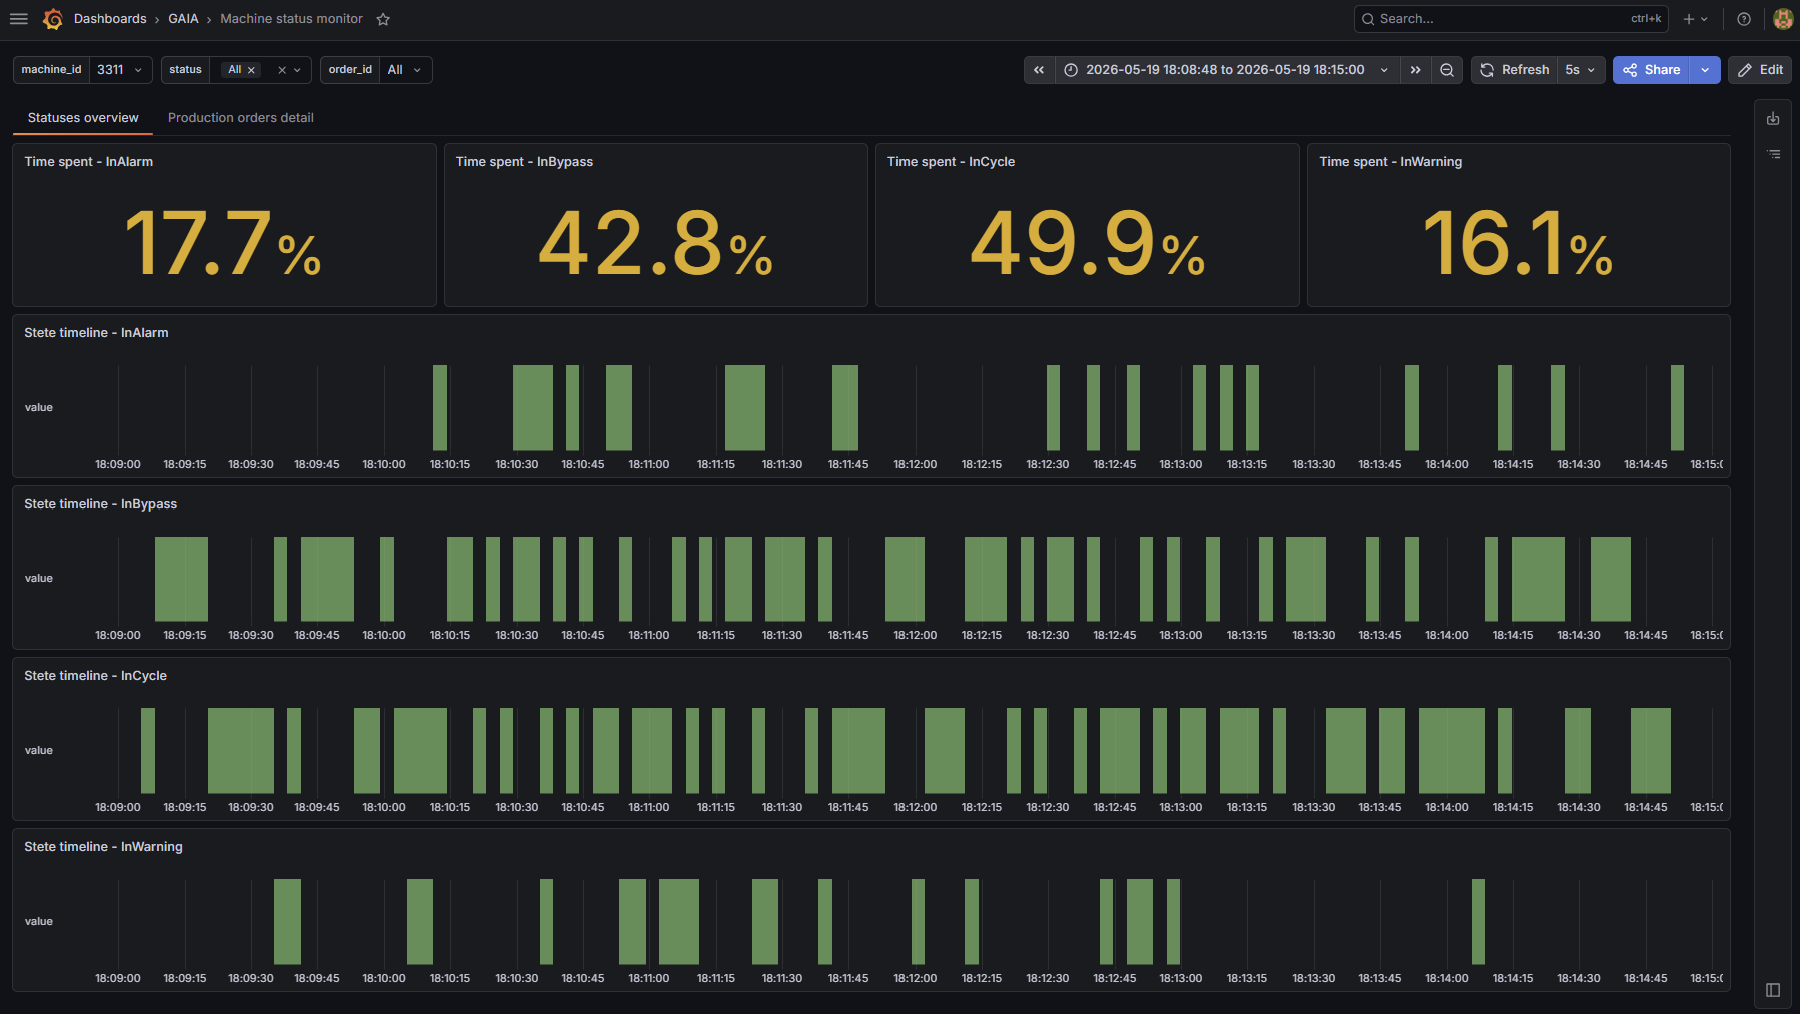
\includegraphics[width=0.8\linewidth]{img/grafana-1.png}
        \caption{Scheda relativa alla panoramica degli stati macchina}
    \end{figure}
    
    \paragraph{Dettaglio ordini di produzione}
    Grazie all'arricchimento dei dati effettuato dal \textit{gateway} tramite le \textsc{api} del \textsc{mes}, questa sezione permette di monitorare l'andamento delle commesse attive nell'intervallo temporale scelto. Sono stati utilizzati:
    \begin{itemize}
        \item \textit{\textbf{Table}}: riassume le informazioni anagrafiche e i metadati degli ordini selezionati;
        \item \textit{\textbf{Time Series}}: visualizza graficamente l'andamento delle quantità prodotte e degli scarti dichiarati durante l'avanzamento della produzione.
    \end{itemize}

    \begin{figure}[htbp]
        \centering
        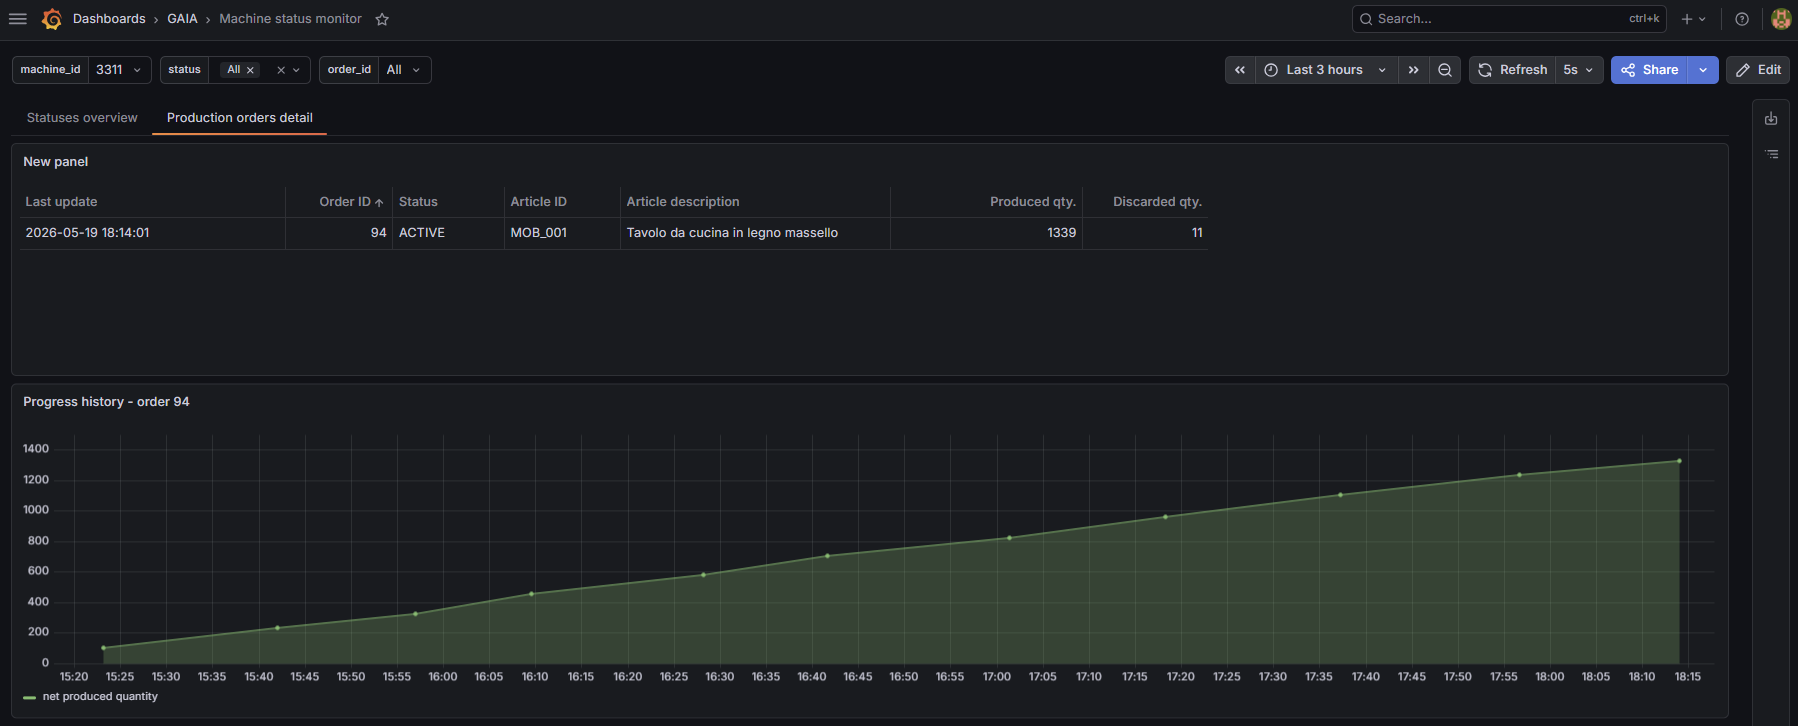
\includegraphics[width=0.8\linewidth]{img/grafana-2.png}
        \caption{Scheda relativa al dettaglio degli ordini di produzione}
    \end{figure}
    
    Nella configurazione attuale, le visualizzazioni adottano i parametri grafici predefiniti, senza l'implementazione di regole di \textit{alerting} o palette di colori personalizzate, focalizzandosi momentaneamente solo sulla correttezza della rappresentazione del dato.

    \section{Rilascio}
    
    Il rilascio del codice è stato ingegnerizzato seguendo metodologie di \textit{Continuous Integration} e \textit{Continuous Deployment} (CI/CD), con l'obiettivo di centralizzare il \textit{deploy} del codice sui \textit{gateway}. Ai fini della simulazione realizzata per la relazione, il medesimo approccio è stato adottato anche per il codice del server \textsc{opc ua}.
    
    \subsection{Pipeline di Build e Registry Centralizzato}
    La creazione e la distribuzione delle immagini Docker sono state automatizzate tramite \textit{GitHub Actions}. Come definito nel file \verb|docker-publish.yml|, il processo si innesca ad ogni \textit{push} sul branch \verb|main| che coinvolga i sorgenti dei microservizi citati sopra.
    
    Sfruttando una \textit{matrix strategy}, la \textit{pipeline} genera in parallelo le immagini per il \textit{gateway} e per il server \textsc{opc ua}, pubblicandole al termine della compilazione sul \textit{GitHub Container Registry} (\textsc{ghcr}).
    Questa scelta progettuale alleggerisce i dispositivi \textit{edge} dall'onere della compilazione locale, riducendo la complessità e i tempi di ogni rilascio.
    
    \subsection{Automazione e Dispiegamento Edge}
    
    L'architettura permette a ogni \textit{gateway} fisico di gestire molteplici macchinari. Le configurazioni di ogni collegamento sono definite in appositi file \verb|.env|, raggruppati in una directory specifica. Il ciclo di vita dei \textit{container} su ogni unità \textit{edge} è regolato da due script Bash.
    
    \paragraph{\texttt{start\_containers.sh}} 
    Lo script è progettato per essere eseguito automaticamente al \textit{boot} del dispositivo. In un contesto di produzione, ciò si ottiene configurando un'unità di servizio \texttt{systemd}, tuttavia, ai fini della presente simulazione, l'esecuzione è stata gestita manualmente. Dopo i controlli di integrità iniziali, lo script scansiona la cartella delle configurazioni e, per ogni file \verb|.env| individuato, istanzia un \textit{container} con le seguenti specifiche:
    \begin{itemize}
        \item \textbf{nome}: coincide con quello del file di configurazione;
        \item \textbf{rete}: viene inserito nella rete Docker \verb|gaia-global-network| per consentire la comunicazione con il broker \textsc{emqx}, il collettore SigNoz e le \textsc{api} del gestionale;
        \item \textbf{resilienza:} applicazione della \textit{policy} \verb|--restart unless-stopped|, che garantisce il riavvio automatico del processo in caso di errore interno o riavvio del demone Docker;
        \item \textbf{sicurezza:} esecuzione in modalità \textit{read-only} per preservare la durata dei supporti di memoria e impedire modifiche non autorizzate al \textit{file system} dei container.
    \end{itemize}
    
    \paragraph{\texttt{stop\_containers.sh}} 
    Eseguito prima dello \textit{shutdown} del sistema, questo script garantisce uno spegnimento controllato dei servizi. Iterando sui file di configurazione attivi, lo script invia un comando per l'arresto e assicura la successiva rimozione dei \textit{container}. In questo modo si garantisce un ambiente pulito ad ogni riavvio. \newline

    Per facilitare la manutenzione e la diagnostica locale, entrambi gli \textit{script} integrano un semplice meccanismo di \textit{logging}, che aggiorna un file di \textit{report} dedicato, registrando l'esito delle operazioni e fornendo una tracciabilità essenziale anche durante le fasi più critiche dell'operatività dei \textit{gateway}.

    \section{Conclusioni}

    Il progetto ha dimostrato con successo la fattibilità di un’infrastruttura IoT agile, resiliente e scalabile per il monitoraggio industriale, capace di trasformare telemetrie grezze in informazioni strutturate, centralizzate e immediatamente fruibili, soddisfacendo sia i requisiti iniziali sia quelli emersi durante lo sviluppo:

    
    \begin{itemize}
        \item \textbf{interoperabilità e standardizzazione}: l'adozione combinata di \textsc{opc ua} e \textsc{mqtt} ha dimostrato come sia possibile astrarre la complessità di un parco macchine eterogeneo, uniformando e rendendo coerente il flusso informativo di fabbrica;
        \item \textbf{portabilità e isolamento}: l'architettura basata su \textit{container} ha garantito il totale disaccoppiamento dall'hardware sottostante, permettendo di scalare rapidamente il monitoraggio su nuovi impianti attraverso semplici modifiche ai file di configurazione;
        \item \textbf{efficienza e manutenibilità}: le soluzioni applicate sui nodi \textit{edge} (come la gestione della memoria in sola lettura) e la centralizzazione dell'osservabilità su SigNoz hanno ridotto l'usura dei supporti fisici e ottimizzato drasticamente i tempi di \textit{troubleshooting}.
    \end{itemize}
        
    Al netto di quanto realizzato, l'intero sistema è stato progettato con una modularità tale da consentire diversi sviluppi futuri. Tra le evoluzioni principali si configurano:
    \begin{itemize}
        \item \textbf{estensione del monitoraggio}: ampliamento del raggio d'azione della piattaforma attraverso l'integrazione di nuovi nodi di campo e metriche di impianto;
        \item \textbf{miglioramento tolleranza ai guasti di rete}: analisi delle performance di rete con l'obiettivo di valutare l'implementazione di meccanismi più robusti per l'invio dei messaggi (come un innalzamento della QoS);
        \item \textbf{configurazione di sistemi di \textit{alerting}}: integrazione su Grafana di regole di notifica automatica al verificarsi di anomalie o stati di allarme prolungati, abilitando una manutenzione più reattiva;
        \item \textbf{\textit{fine-tuning} e analisi delle prestazioni}: esecuzione di test di carico sulla base di dati per calibrare i parametri di partizionamento dei \textit{chunk} ed esaminando, se necessario, soluzioni di \textit{storage} alternative o complementari per scopi analitici;
        \item \textbf{\textit{machine learning} per manutenzione predittiva}: applicazione di algoritmi di \textit{Machine Learning} sullo storico delle variazioni, volti a identificare \textit{trend} di deriva e prevenire i fermi macchina in relazione a specifici articoli e volumi produttivi.
        \item \textbf{documentazione e ciclo di vita del software}: introduzione di strumenti per la generazione automatica e la pubblicazione della documentazione tecnica del codice, ottimizzando ulteriormente la gestione delle pipeline di CI/CD;
    \end{itemize}
    
\end{document}
